
\section{Vorwort}
\label{vorwort}
	\begin{multicols}{2}
	\subsection*{Willkommen in der Informatik!}	

	Das neue Semester an der TU Braunschweig beginnt und du bist dabei. Die Fachgruppe Informatik (s. Seite \pageref{fachgruppe}) begrüßt dich ganz herzlich an der Uni und möchte dir mit der "1-ten" den Start vereinfachen. Diese Erstsemesterzeitung der Informatiker soll dir dabei helfen, Antworten auf viele Fragen, die sich zu Beginn des Studiums stellen, zu beantworten.

	\subsubsection*{Aufbau dieses Heftes}
		Der Fokus der ersten Seiten liegt auf den vielen Fragen zum Studienbeginn, deinem Studiengang und der Infrastruktur der Uni. Wir erklären, wie Studienplanung funktioniert und was für Bachelor und Master wichtig ist.
Der Fachgruppenrat Informatik stellt sich vor und beantwortet die Fragen, wer er ist und was er macht. 
\columnbreak
	\subsubsection*{Der Blog}
		Der Fachgruppenrat Informatik betreibt den Blog FGInfo (\url{http://fginfo.cs.tu-bs.de}). Dort werden unsere Termine und Veranstaltungen, z.B. Spieleabende, angekündigt und über die hochschulpolitische Arbeit berichtet.
Zusätzlich bietet diese Seite viele Infos, Tipps und Wissenswertes rund um die Informatik-Studiengänge.
Dieses Heft, die 1-te, gibt es dort auch noch einmal zu finden. Mitunter
ergeben sich noch nach dem Druck Änderungen, gerade bei Terminen, also schau auf jeden Fall dort rein!

	\vspace*{0.5cm}

	Viel Spaß und Erfolg im  Studium wünscht  die\\
	\hspace*{2cm}Fachgruppe Informatik
	\end{multicols}
	\vspace{0.5cm}
	\begin{center} 
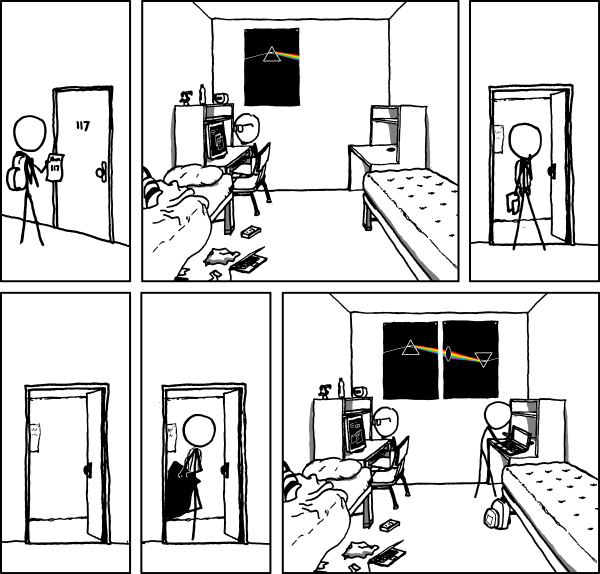
\includegraphics[totalheight=12cm]{bilder/XKCD/dorm_poster}
\end{center}
